\chapter{Implementation, Results and Discussions}

\section{Introduction}
This chapter reports how the four detector configurations of Chapter~III were
trained and evaluated, and what the measurements show. It first fixes the
experimental setup and the evaluation metrics, then describes the C2A dataset and
its split. The results are presented in two parts: a quantitative comparison of
the additive ablation on the C2A test set, and a qualitative analysis of where the
recommended model succeeds and fails. The chapter closes with a comparison against
published results on the same dataset, the inference-time and lightweight
extensions, a check of the stated objectives, and a short cost account.

\section{Experimental Setup}
All models were trained and evaluated on a single workstation with an NVIDIA RTX
4070 Ti SUPER (16~GB, Ada, compute capability 8.9), an Intel Core i7-14700K, and
128~GB of RAM, running Windows~11. The software stack was Python~3.11.9,
PyTorch~2.12.0 (CUDA~12.6, cuDNN~9.10), and Ultralytics~8.4.56, with
pycocotools for COCO-style evaluation. Training used a single GPU with no
distributed data parallelism. Table~\ref{tab:setup} lists the training
configuration; it is identical across the four models so that any measured
difference is due to the architecture, not the optimiser.

\begin{table}[tbp]
  \centering
  \caption{Training configuration, held identical across all four configurations.
  Batch size was set to 16 with an out-of-memory retry ladder; the P2-head models
  settled at 8 because the added stride-4 scale raises activation memory.}
  \label{tab:setup}
  \begin{tabular}{@{}l l@{}}
    \toprule
    Setting & Value \\
    \midrule
    Input resolution & $640 \times 640$ (letterbox) \\
    Optimiser & AdamW, $\text{lr}_0 = 0.001$, $\text{lr}_f = 0.01$, cosine schedule \\
    Epochs (max) & 300, early stop on fitness (patience 50) and F2 (patience 40) \\
    Batch size & 16 (baseline, CBAM); 8 (P2-head models, via OOM ladder) \\
    Mixed precision & enabled (AMP) \\
    Augmentation & YOLO11 defaults; \texttt{close\_mosaic} = 10; no copy--paste/mixup \\
    Seed & 0 (deterministic cuDNN) \\
    \bottomrule
  \end{tabular}
\end{table}

\section{Evaluation Metrics}
Because the task is finding people in disaster imagery, recall is weighted more
heavily than precision: a missed victim is costlier than a false alarm that an
operator can dismiss. The primary operating metric is therefore the $F_2$ score,
which weights recall four times as heavily as precision. With true positives
$\mathit{TP}$, false positives $\mathit{FP}$, and false negatives $\mathit{FN}$
(a detection counts as $\mathit{TP}$ when its intersection-over-union with a
ground-truth box is at least $0.5$), precision $P$, recall $R$, and the
$F_\beta$ family are
\begin{align}
  P = \frac{\mathit{TP}}{\mathit{TP}+\mathit{FP}}, \qquad
  R = \frac{\mathit{TP}}{\mathit{TP}+\mathit{FN}}, \qquad
  F_\beta = (1+\beta^{2})\,\frac{P \cdot R}{\beta^{2} P + R},
\end{align}
with $\beta = 1$ for $F_1$ and $\beta = 2$ for $F_2$. Localisation quality is
measured by COCO~\cite{lin2014coco} average precision: $\mathrm{AP}$ averaged over
IoU thresholds $0.5$ to $0.95$, along with $\mathrm{AP}_{50}$, $\mathrm{AP}_{75}$,
and the small-object $\mathrm{AP}_S$. Because the targets are extremely small, recall is
also reported per object-size band (very-tiny $<8$~px, tiny $8$--$16$~px,
small $16$--$32$~px, and medium $32$--$96$~px), which is where the effect of
the P2 head is visible. Efficiency is reported as parameter count, GFLOPs, and
end-to-end latency measured on the 4070 Ti SUPER. AP-style metrics use
$\text{conf} = 0.001$, $\text{IoU} = 0.7$; operational $F_1$/$F_2$ use the
confidence threshold that maximises each score.

\section{Dataset}
The models are trained and tested on C2A (Combination to Application), a dataset
for human detection in disaster scenes~\cite{nihal2024c2a}. C2A is semi-synthetic:
disaster backgrounds from AIDER are combined with human poses segmented from
pose-estimation datasets by a U$^2$-Net model, which are then randomly scaled and
placed and annotated with horizontal bounding boxes. The dataset contains 10{,}215
images and roughly 360{,}000 labelled human instances across four scene types
(collapsed buildings, fire, flood, and traffic accident). Targets are dominated by
very small objects: about 47\% of people occupy fewer than 10~px and about 52\%
fall between 10 and 50~px. All pose sub-labels are collapsed to a single
\texttt{person} class; the C2A annotation stores this class under a numeric
placeholder, which is mapped to \texttt{person} at load time. The frozen split
used throughout this thesis is given in Table~\ref{tab:split}; the split hashes are
recorded so that every model sees exactly the same images.

\begin{table}[tbp]
  \centering
  \caption{C2A split used for all experiments. The same frozen split (verified by
  MD5) is used by every configuration.}
  \label{tab:split}
  \begin{tabular}{@{}l r r r@{}}
    \toprule
    & Train & Validation & Test \\
    \midrule
    Images & 6{,}129 & 2{,}043 & 2{,}043 \\
    \bottomrule
  \end{tabular}
\end{table}

Representative samples covering all four scene types and the range of target
scales are shown in Figure~\ref{fig:dataset_samples}.

\begin{figure}[tbp]
  \centering
  \begin{minipage}{0.44\linewidth}\centering
    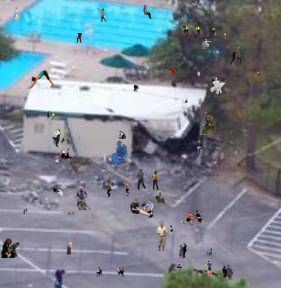
\includegraphics[width=\linewidth,height=3.7cm,keepaspectratio]{figures/c2a_collapsed.png}\\[2pt]
    {\small (a) collapsed building}
  \end{minipage}\hfill
  \begin{minipage}{0.44\linewidth}\centering
    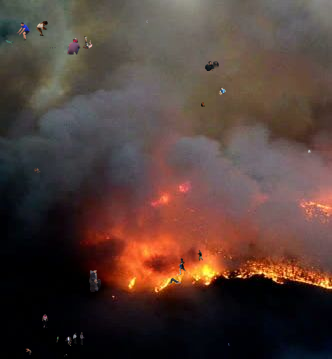
\includegraphics[width=\linewidth,height=3.7cm,keepaspectratio]{figures/c2a_fire.png}\\[2pt]
    {\small (b) fire}
  \end{minipage}\\[8pt]
  \begin{minipage}{0.44\linewidth}\centering
    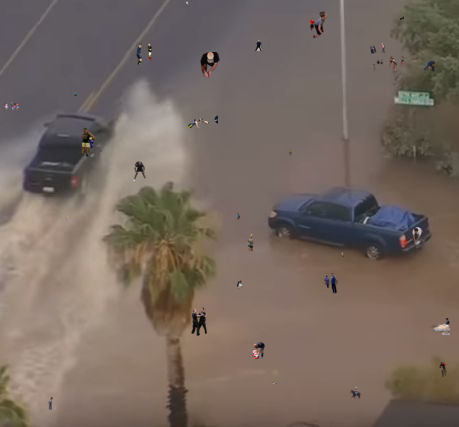
\includegraphics[width=\linewidth,height=3.7cm,keepaspectratio]{figures/c2a_flood.png}\\[2pt]
    {\small (c) flood}
  \end{minipage}\hfill
  \begin{minipage}{0.44\linewidth}\centering
    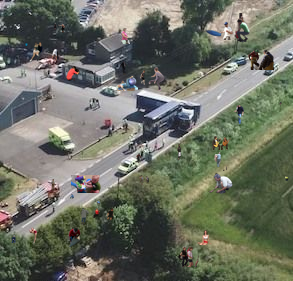
\includegraphics[width=\linewidth,height=3.7cm,keepaspectratio]{figures/c2a_traffic.png}\\[2pt]
    {\small (d) traffic incident}
  \end{minipage}
  \caption{Representative C2A test samples, one per scene type: (a)~collapsed
  building, (b)~fire, (c)~flood, and (d)~traffic incident. Human targets are small
  and numerous in every scene, which is the central difficulty of the dataset.}
  \label{fig:dataset_samples}
\end{figure}

The severity of that difficulty is quantified in Figure~\ref{fig:sizedist}: on the
test split, $99.6\%$ of the human instances are smaller than $32$~px and about a
third are below $8$~px, so the two coarsest detection scales (P4 and P5) cover almost
no targets and the small-object scales dominate.

\begin{figure}[tbp]
  \centering
  % ============================================================================
%  fig_size_distribution.tex -- C2A test-set human-size distribution (real counts).
%  Counts from runs_sahi_tta baseline_640 per_size_gt_count (sqrt-area bins,
%  2,043 test images, 72,523 instances). Needs \usepackage{tikz} (+ amsmath).
%  Include with:  % ============================================================================
%  fig_size_distribution.tex -- C2A test-set human-size distribution (real counts).
%  Counts from runs_sahi_tta baseline_640 per_size_gt_count (sqrt-area bins,
%  2,043 test images, 72,523 instances). Needs \usepackage{tikz} (+ amsmath).
%  Include with:  % ============================================================================
%  fig_size_distribution.tex -- C2A test-set human-size distribution (real counts).
%  Counts from runs_sahi_tta baseline_640 per_size_gt_count (sqrt-area bins,
%  2,043 test images, 72,523 instances). Needs \usepackage{tikz} (+ amsmath).
%  Include with:  \input{tikz/fig_size_distribution}
%  y = count * 0.00015 cm   (20,000 instances -> 3 cm)
% ============================================================================
\definecolor{sdBlueFill}{HTML}{DAE8FC}
\definecolor{sdBlueStroke}{HTML}{6C8EBF}
\definecolor{sdRedFill}{HTML}{F8CECC}
\definecolor{sdRedStroke}{HTML}{B85450}
\definecolor{sdGrey}{HTML}{888888}
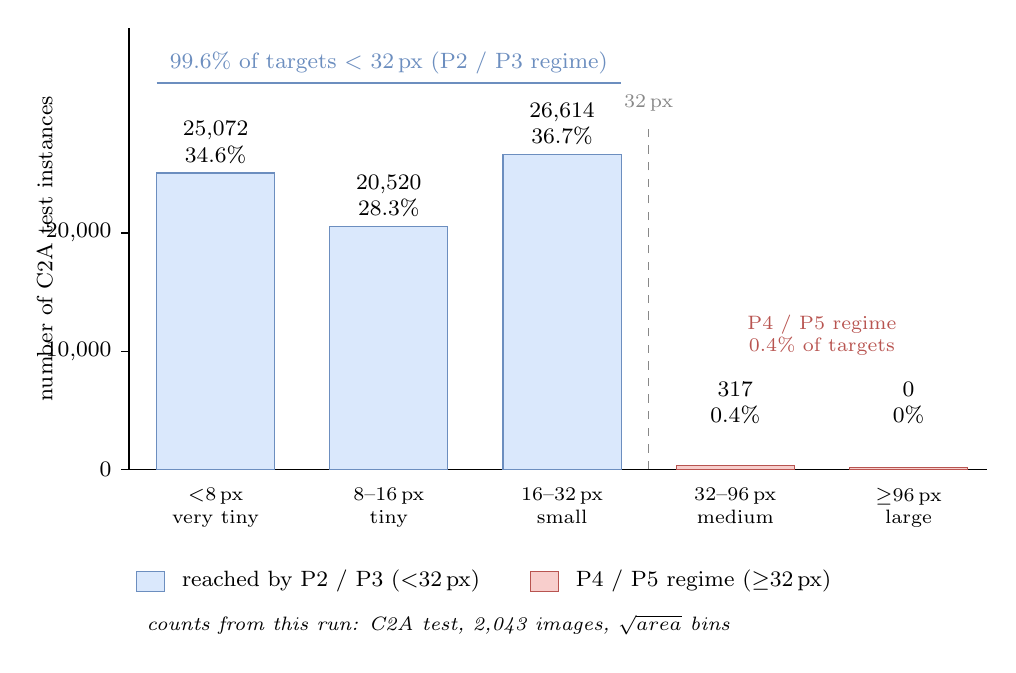
\begin{tikzpicture}[font=\footnotesize]
  % ---- axes ----
  \draw[black] (0.9,0) -- (0.9,5.6);
  \draw[black] (0.9,0) -- (11.8,0);
  \foreach \c/\y in {0/0, 10{,}000/1.5, 20{,}000/3.0}{%
    \draw[black] (0.8,\y) -- (0.9,\y);
    \node[left] at (0.8,\y) {\c};
  }
  \node[rotate=90,anchor=south] at (0.05,2.8) {number of C2A test instances};

  % ---- 32 px boundary (between small and medium) ----
  \draw[sdGrey,dashed] (7.5,0) -- (7.5,4.4);
  \node[sdGrey,font=\scriptsize,anchor=south] at (7.5,4.42) {32\,px};

  % ---- bars: blue (<32 px, P2/P3 regime), red (>=32 px, P4/P5 regime) ----
  \filldraw[fill=sdBlueFill,draw=sdBlueStroke] (1.25,0) rectangle (2.75,3.7608);
  \filldraw[fill=sdBlueFill,draw=sdBlueStroke] (3.45,0) rectangle (4.95,3.0780);
  \filldraw[fill=sdBlueFill,draw=sdBlueStroke] (5.65,0) rectangle (7.15,3.9921);
  \filldraw[fill=sdRedFill,draw=sdRedStroke]   (7.85,0) rectangle (9.35,0.0476);
  \filldraw[fill=sdRedFill,draw=sdRedStroke]   (10.05,0) rectangle (11.55,0.02);

  % ---- count + percent above each bar ----
  \node[above,align=center] at (2.0,3.7608) {25{,}072\\34.6\%};
  \node[above,align=center] at (4.2,3.0780) {20{,}520\\28.3\%};
  \node[above,align=center] at (6.4,3.9921) {26{,}614\\36.7\%};
  \node[above,align=center] at (8.6,0.45)   {317\\0.4\%};
  \node[above,align=center] at (10.8,0.45)  {0\\0\%};

  % ---- x labels: size range + class ----
  \node[below,align=center,font=\scriptsize] at (2.0,-0.12)  {$<$8\,px\\very tiny};
  \node[below,align=center,font=\scriptsize] at (4.2,-0.12)  {8--16\,px\\tiny};
  \node[below,align=center,font=\scriptsize] at (6.4,-0.12)  {16--32\,px\\small};
  \node[below,align=center,font=\scriptsize] at (8.6,-0.12)  {32--96\,px\\medium};
  \node[below,align=center,font=\scriptsize] at (10.8,-0.12) {$\geq$96\,px\\large};

  % ---- annotations ----
  \draw[sdBlueStroke,thick] (1.25,4.9) -- (7.15,4.9);
  \node[above,text=sdBlueStroke] at (4.2,4.9) {99.6\% of targets $<$ 32\,px  (P2 / P3 regime)};
  \node[align=center,text=sdRedStroke,font=\scriptsize] at (9.7,1.7) {P4 / P5 regime\\0.4\% of targets};

  % ---- legend ----
  \filldraw[fill=sdBlueFill,draw=sdBlueStroke] (1.0,-1.55) rectangle (1.35,-1.30);
  \node[anchor=west] at (1.45,-1.425) {reached by P2 / P3 ($<$32\,px)};
  \filldraw[fill=sdRedFill,draw=sdRedStroke] (6.0,-1.55) rectangle (6.35,-1.30);
  \node[anchor=west] at (6.45,-1.425) {P4 / P5 regime ($\geq$32\,px)};
  \node[anchor=west,font=\itshape\scriptsize] at (1.0,-1.98)
        {counts from this run: C2A test, 2{,}043 images, $\sqrt{\text{area}}$ bins};
\end{tikzpicture}

%  y = count * 0.00015 cm   (20,000 instances -> 3 cm)
% ============================================================================
\definecolor{sdBlueFill}{HTML}{DAE8FC}
\definecolor{sdBlueStroke}{HTML}{6C8EBF}
\definecolor{sdRedFill}{HTML}{F8CECC}
\definecolor{sdRedStroke}{HTML}{B85450}
\definecolor{sdGrey}{HTML}{888888}
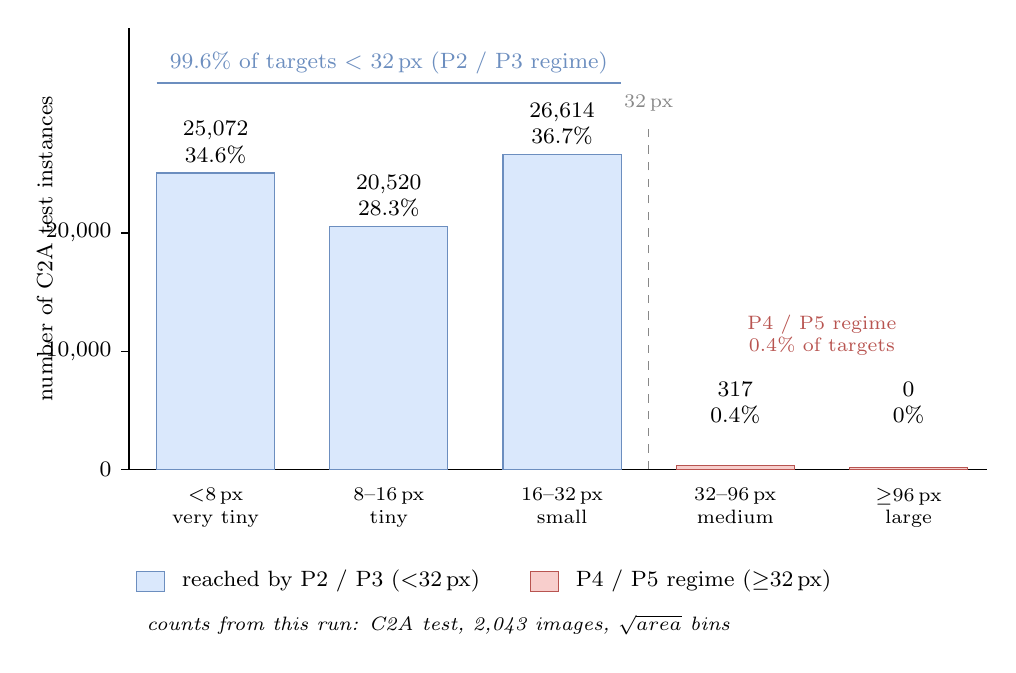
\begin{tikzpicture}[font=\footnotesize]
  % ---- axes ----
  \draw[black] (0.9,0) -- (0.9,5.6);
  \draw[black] (0.9,0) -- (11.8,0);
  \foreach \c/\y in {0/0, 10{,}000/1.5, 20{,}000/3.0}{%
    \draw[black] (0.8,\y) -- (0.9,\y);
    \node[left] at (0.8,\y) {\c};
  }
  \node[rotate=90,anchor=south] at (0.05,2.8) {number of C2A test instances};

  % ---- 32 px boundary (between small and medium) ----
  \draw[sdGrey,dashed] (7.5,0) -- (7.5,4.4);
  \node[sdGrey,font=\scriptsize,anchor=south] at (7.5,4.42) {32\,px};

  % ---- bars: blue (<32 px, P2/P3 regime), red (>=32 px, P4/P5 regime) ----
  \filldraw[fill=sdBlueFill,draw=sdBlueStroke] (1.25,0) rectangle (2.75,3.7608);
  \filldraw[fill=sdBlueFill,draw=sdBlueStroke] (3.45,0) rectangle (4.95,3.0780);
  \filldraw[fill=sdBlueFill,draw=sdBlueStroke] (5.65,0) rectangle (7.15,3.9921);
  \filldraw[fill=sdRedFill,draw=sdRedStroke]   (7.85,0) rectangle (9.35,0.0476);
  \filldraw[fill=sdRedFill,draw=sdRedStroke]   (10.05,0) rectangle (11.55,0.02);

  % ---- count + percent above each bar ----
  \node[above,align=center] at (2.0,3.7608) {25{,}072\\34.6\%};
  \node[above,align=center] at (4.2,3.0780) {20{,}520\\28.3\%};
  \node[above,align=center] at (6.4,3.9921) {26{,}614\\36.7\%};
  \node[above,align=center] at (8.6,0.45)   {317\\0.4\%};
  \node[above,align=center] at (10.8,0.45)  {0\\0\%};

  % ---- x labels: size range + class ----
  \node[below,align=center,font=\scriptsize] at (2.0,-0.12)  {$<$8\,px\\very tiny};
  \node[below,align=center,font=\scriptsize] at (4.2,-0.12)  {8--16\,px\\tiny};
  \node[below,align=center,font=\scriptsize] at (6.4,-0.12)  {16--32\,px\\small};
  \node[below,align=center,font=\scriptsize] at (8.6,-0.12)  {32--96\,px\\medium};
  \node[below,align=center,font=\scriptsize] at (10.8,-0.12) {$\geq$96\,px\\large};

  % ---- annotations ----
  \draw[sdBlueStroke,thick] (1.25,4.9) -- (7.15,4.9);
  \node[above,text=sdBlueStroke] at (4.2,4.9) {99.6\% of targets $<$ 32\,px  (P2 / P3 regime)};
  \node[align=center,text=sdRedStroke,font=\scriptsize] at (9.7,1.7) {P4 / P5 regime\\0.4\% of targets};

  % ---- legend ----
  \filldraw[fill=sdBlueFill,draw=sdBlueStroke] (1.0,-1.55) rectangle (1.35,-1.30);
  \node[anchor=west] at (1.45,-1.425) {reached by P2 / P3 ($<$32\,px)};
  \filldraw[fill=sdRedFill,draw=sdRedStroke] (6.0,-1.55) rectangle (6.35,-1.30);
  \node[anchor=west] at (6.45,-1.425) {P4 / P5 regime ($\geq$32\,px)};
  \node[anchor=west,font=\itshape\scriptsize] at (1.0,-1.98)
        {counts from this run: C2A test, 2{,}043 images, $\sqrt{\text{area}}$ bins};
\end{tikzpicture}

%  y = count * 0.00015 cm   (20,000 instances -> 3 cm)
% ============================================================================
\definecolor{sdBlueFill}{HTML}{DAE8FC}
\definecolor{sdBlueStroke}{HTML}{6C8EBF}
\definecolor{sdRedFill}{HTML}{F8CECC}
\definecolor{sdRedStroke}{HTML}{B85450}
\definecolor{sdGrey}{HTML}{888888}
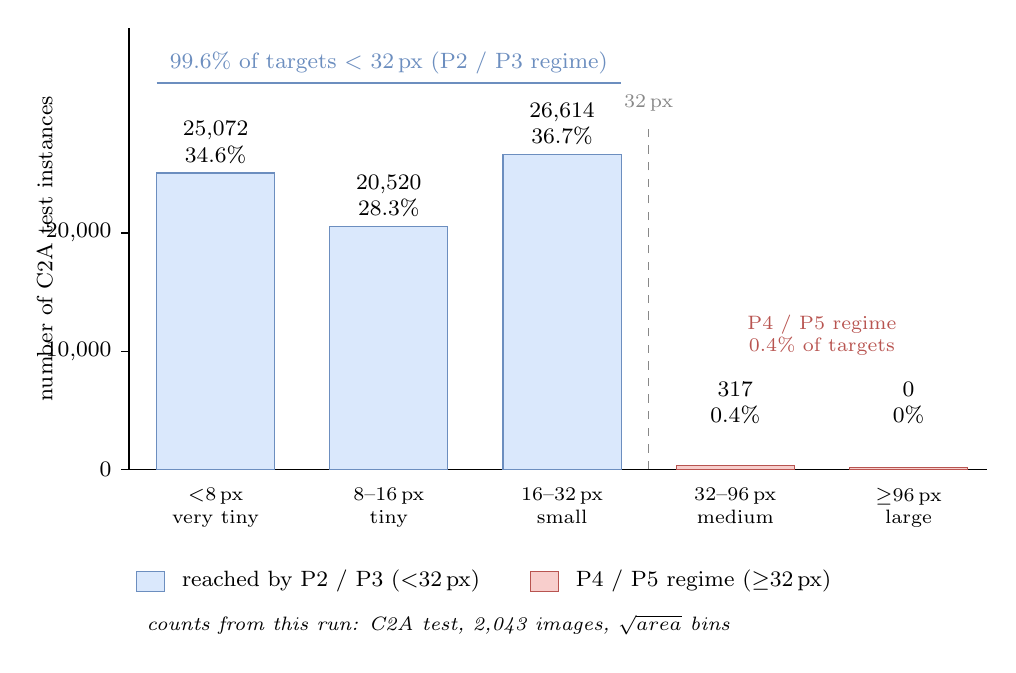
\begin{tikzpicture}[font=\footnotesize]
  % ---- axes ----
  \draw[black] (0.9,0) -- (0.9,5.6);
  \draw[black] (0.9,0) -- (11.8,0);
  \foreach \c/\y in {0/0, 10{,}000/1.5, 20{,}000/3.0}{%
    \draw[black] (0.8,\y) -- (0.9,\y);
    \node[left] at (0.8,\y) {\c};
  }
  \node[rotate=90,anchor=south] at (0.05,2.8) {number of C2A test instances};

  % ---- 32 px boundary (between small and medium) ----
  \draw[sdGrey,dashed] (7.5,0) -- (7.5,4.4);
  \node[sdGrey,font=\scriptsize,anchor=south] at (7.5,4.42) {32\,px};

  % ---- bars: blue (<32 px, P2/P3 regime), red (>=32 px, P4/P5 regime) ----
  \filldraw[fill=sdBlueFill,draw=sdBlueStroke] (1.25,0) rectangle (2.75,3.7608);
  \filldraw[fill=sdBlueFill,draw=sdBlueStroke] (3.45,0) rectangle (4.95,3.0780);
  \filldraw[fill=sdBlueFill,draw=sdBlueStroke] (5.65,0) rectangle (7.15,3.9921);
  \filldraw[fill=sdRedFill,draw=sdRedStroke]   (7.85,0) rectangle (9.35,0.0476);
  \filldraw[fill=sdRedFill,draw=sdRedStroke]   (10.05,0) rectangle (11.55,0.02);

  % ---- count + percent above each bar ----
  \node[above,align=center] at (2.0,3.7608) {25{,}072\\34.6\%};
  \node[above,align=center] at (4.2,3.0780) {20{,}520\\28.3\%};
  \node[above,align=center] at (6.4,3.9921) {26{,}614\\36.7\%};
  \node[above,align=center] at (8.6,0.45)   {317\\0.4\%};
  \node[above,align=center] at (10.8,0.45)  {0\\0\%};

  % ---- x labels: size range + class ----
  \node[below,align=center,font=\scriptsize] at (2.0,-0.12)  {$<$8\,px\\very tiny};
  \node[below,align=center,font=\scriptsize] at (4.2,-0.12)  {8--16\,px\\tiny};
  \node[below,align=center,font=\scriptsize] at (6.4,-0.12)  {16--32\,px\\small};
  \node[below,align=center,font=\scriptsize] at (8.6,-0.12)  {32--96\,px\\medium};
  \node[below,align=center,font=\scriptsize] at (10.8,-0.12) {$\geq$96\,px\\large};

  % ---- annotations ----
  \draw[sdBlueStroke,thick] (1.25,4.9) -- (7.15,4.9);
  \node[above,text=sdBlueStroke] at (4.2,4.9) {99.6\% of targets $<$ 32\,px  (P2 / P3 regime)};
  \node[align=center,text=sdRedStroke,font=\scriptsize] at (9.7,1.7) {P4 / P5 regime\\0.4\% of targets};

  % ---- legend ----
  \filldraw[fill=sdBlueFill,draw=sdBlueStroke] (1.0,-1.55) rectangle (1.35,-1.30);
  \node[anchor=west] at (1.45,-1.425) {reached by P2 / P3 ($<$32\,px)};
  \filldraw[fill=sdRedFill,draw=sdRedStroke] (6.0,-1.55) rectangle (6.35,-1.30);
  \node[anchor=west] at (6.45,-1.425) {P4 / P5 regime ($\geq$32\,px)};
  \node[anchor=west,font=\itshape\scriptsize] at (1.0,-1.98)
        {counts from this run: C2A test, 2{,}043 images, $\sqrt{\text{area}}$ bins};
\end{tikzpicture}

  \caption{Distribution of human-target sizes in the C2A test set ($\sqrt{\text{area}}$
  bins, 2{,}043 images). Bars below $32$~px (blue) fall in the stride-4/8 (P2/P3)
  regime; the coarse P4/P5 heads serve only the $0.4\%$ of targets above $32$~px.}
  \label{fig:sizedist}
\end{figure}

\section{Implementation and Results}

\subsection{Detector Family Benchmark}
Before the ablation, the YOLOv9~\cite{wang2024yolov9}, YOLOv10~\cite{wang2024yolov10},
and YOLO11~\cite{jocher2024yolo11} families were benchmarked on C2A to select a
baseline; the comparison is given in Table~\ref{tab:detbench}. This benchmark was run
under an earlier protocol, so its absolute values are not directly comparable to the
final ablation of Table~\ref{tab:main}; it is used only to choose the backbone. The
largest model, YOLOv9-e, gives the highest accuracy (mAP50 $0.855$, mAP50-95 $0.619$)
but at $111.8$~MB, about three times the size of the mid-size models. YOLO11m
reaches mAP50 $0.841$ and mAP50-95 $0.592$ at $38.6$~MB, close to the best while
staying small enough to deploy, and gives the best accuracy per megabyte of the
family. It was therefore chosen as the baseline.

\begin{table}[tbp]
  \centering
  \caption{Preliminary detector-family benchmark on C2A (test set) used to select
  the baseline. YOLO11m was chosen for its accuracy-to-size balance.}
  \label{tab:detbench}
  \setlength{\tabcolsep}{5pt}
  \begin{tabular}{@{}l r r r r r r@{}}
    \toprule
    Model & mAP50 & mAP50-95 & $P$ & $R$ & $F_1$ & Size (MB) \\
    \midrule
    YOLOv9-s   & 0.787 & 0.504 & 0.841 & 0.736 & 0.785 & 14.5 \\
    YOLOv9-m   & 0.823 & 0.565 & 0.863 & 0.772 & 0.815 & 38.9 \\
    YOLOv9-e   & \textbf{0.855} & \textbf{0.619} & \textbf{0.884} & \textbf{0.805} & \textbf{0.843} & 111.8 \\
    YOLOv10-s  & 0.792 & 0.517 & 0.836 & 0.738 & 0.784 & 15.8 \\
    YOLOv10-m  & 0.827 & 0.571 & 0.857 & 0.777 & 0.815 & 31.9 \\
    YOLOv10-l  & 0.843 & 0.598 & 0.870 & 0.792 & 0.829 & 49.8 \\
    YOLOv11-s  & 0.803 & 0.535 & 0.845 & 0.757 & 0.798 & 18.3 \\
    \textbf{YOLO11m (selected)} & 0.841 & 0.592 & 0.867 & 0.794 & 0.829 & 38.6 \\
    YOLOv11-l  & 0.847 & 0.603 & 0.876 & 0.796 & 0.834 & 48.8 \\
    \bottomrule
  \end{tabular}
\end{table}

\subsection{Attention Module Selection}
The choice of CBAM over the lighter ECA module~\cite{wang2020eca} was settled by a
preliminary comparison on the baseline, summarised in Table~\ref{tab:eca} (again an
earlier protocol; values are relative, not comparable to Table~\ref{tab:main}).
Replacing the baseline attention with CBAM gave the highest $F_2$ ($0.849$) and the
highest small-object recall ($0.892$, $+1.3$ points over the baseline), whereas ECA
barely moved either metric. CBAM also reduced parameters relative to the baseline
block. CBAM was therefore adopted as the attention module and carried into the main
ablation.

\begin{table}[tbp]
  \centering
  \caption{Preliminary attention-module comparison on C2A (earlier protocol).
  CBAM gives the best $F_2$ and small-object recall, so it is used in the ablation.}
  \label{tab:eca}
  \begin{tabular}{@{}l r r r@{}}
    \toprule
    Model & $F_2$ & Small-object recall & $F_1$ \\
    \midrule
    YOLO11m baseline & 0.844 & 0.881 & 0.837 \\
    + ECA            & 0.844 & 0.884 & 0.840 \\
    + CBAM           & \textbf{0.849} & \textbf{0.892} & \textbf{0.842} \\
    \bottomrule
  \end{tabular}
\end{table}

\subsection{Quantitative Results}
Table~\ref{tab:main} reports the four configurations on the C2A test set under the
COCO protocol. Aggregate average precision is saturated: all four models sit within
$0.002$ AP of one another. The differences appear in the metrics that matter for
this task. Adding the P2 head raises $\mathrm{AP}_{50}$ from $0.843$ to $0.853$,
$\mathrm{AR}_{100}$ from $0.691$ to $0.703$, and the operational $F_2$ from
$0.840$ to $0.844$, at a cost of about $0.5$~M parameters and $1$~ms of latency.
CBAM on its own is close to free: it removes about $1$~M parameters relative to the
baseline (it replaces the two heavier C2PSA blocks) while matching or slightly
improving $F_1$/$F_2$ and giving the lowest latency of the four. The state-space
neck is the outlier in the wrong direction: it adds $2.4$~M parameters and roughly
triples end-to-end latency ($14.6 \to 41.1$~ms) without improving any accuracy
metric. On this evidence the recommended configuration is CBAM~+~P2, and the
state-space neck is not carried forward.

\begin{table}[tbp]
  \centering
  \caption{Additive ablation on the C2A test set (COCO protocol). AP is averaged
  over IoU 0.5--0.95; $F_1$ and $F_2$ are at their optimal confidence thresholds;
  latency is end-to-end on the RTX 4070 Ti SUPER. Best value in each column in bold.}
  \label{tab:main}
  \setlength{\tabcolsep}{4pt}
  \begin{tabular}{@{}l r r r r r r r r r@{}}
    \toprule
    Model & Params & GFLOPs & AP & $\mathrm{AP}_{50}$ & $\mathrm{AP}_{75}$ & $\mathrm{AR}_{100}$ & $F_1$ & $F_2$ & Lat.\ (ms) \\
    & (M) & & & & & & & & \\
    \midrule
    YOLO11m baseline    & 20.03 & 67.7 & \textbf{0.615} & 0.843 & 0.655 & 0.691 & \textbf{0.850} & 0.840 & 13.7 \\
    + CBAM              & 19.08 & 66.9 & \textbf{0.616} & 0.847 & 0.656 & 0.692 & \textbf{0.850} & 0.841 & \textbf{13.5} \\
    + CBAM + P2         & 19.57 & 86.7 & 0.615 & \textbf{0.853} & 0.660 & 0.703 & 0.848 & \textbf{0.844} & 14.6 \\
    + Mamba + CBAM + P2 & 22.01 & 98.4 & 0.614 & 0.852 & \textbf{0.662} & \textbf{0.704} & 0.846 & \textbf{0.844} & 41.1 \\
    \bottomrule
  \end{tabular}
\end{table}

\begin{figure}[tbp]
  \centering
  % ============================================================================
%  fig_ablation_waterfall.tex  --  additive-ablation waterfall on AP50 (TikZ).
%  Colours match the draw.io / Gemini version exactly (HEX below).
%  Needs \usepackage{tikz} in the preamble (added to thesisstyle.sty).
%  Include with:  % ============================================================================
%  fig_ablation_waterfall.tex  --  additive-ablation waterfall on AP50 (TikZ).
%  Colours match the draw.io / Gemini version exactly (HEX below).
%  Needs \usepackage{tikz} in the preamble (added to thesisstyle.sty).
%  Include with:  % ============================================================================
%  fig_ablation_waterfall.tex  --  additive-ablation waterfall on AP50 (TikZ).
%  Colours match the draw.io / Gemini version exactly (HEX below).
%  Needs \usepackage{tikz} in the preamble (added to thesisstyle.sty).
%  Include with:  \input{tikz/fig_ablation_waterfall}
%  y = (AP50 - 0.838) * 333.333 cm  (axis zoomed to 0.838-0.856)
% ============================================================================
\definecolor{wfBaseFill}{HTML}{DAE8FC}
\definecolor{wfBaseStroke}{HTML}{6C8EBF}
\definecolor{wfGainFill}{HTML}{D5E8D4}
\definecolor{wfGainStroke}{HTML}{82B366}
\definecolor{wfRedEdge}{HTML}{FF0000}
\definecolor{wfMambaFill}{HTML}{F8CECC}
\definecolor{wfMambaStroke}{HTML}{B85450}
\definecolor{wfGreenText}{HTML}{2D7D2D}
\definecolor{wfRedText}{HTML}{C00000}
\definecolor{wfGrey}{HTML}{999999}
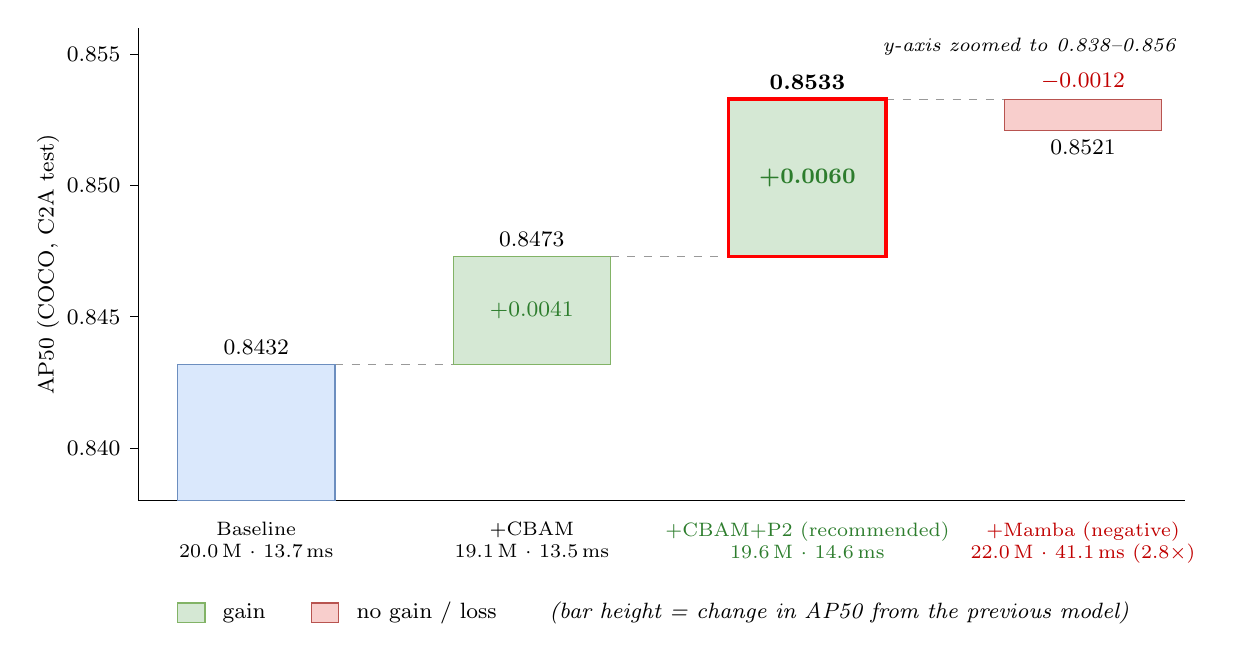
\begin{tikzpicture}[font=\footnotesize]
  % ---- axes ----
  \draw[black] (1.0,0) -- (1.0,6.0);
  \draw[black] (1.0,0) -- (14.3,0);
  \foreach \y/\lab in {0.6667/0.840, 2.3333/0.845, 4.0/0.850, 5.6667/0.855}{%
    \draw[black] (0.9,\y) -- (1.0,\y);
    \node[left] at (0.9,\y) {\lab};
  }
  \node[rotate=90,anchor=south] at (0.12,3.0) {AP50 (COCO, C2A test)};
  \node[anchor=north east,font=\itshape\scriptsize] at (14.3,6.0) {y-axis zoomed to 0.838--0.856};

  % ---- dashed step connectors ----
  \draw[wfGrey,dashed] (3.5,1.7333) -- (5.0,1.7333);
  \draw[wfGrey,dashed] (7.0,3.1)    -- (8.5,3.1);
  \draw[wfGrey,dashed] (10.5,5.1)   -- (12.0,5.1);

  % ---- bars ----
  \filldraw[fill=wfBaseFill,draw=wfBaseStroke]                     (1.5,0)      rectangle (3.5,1.7333);
  \filldraw[fill=wfGainFill,draw=wfGainStroke]                     (5.0,1.7333) rectangle (7.0,3.1);
  \filldraw[fill=wfGainFill,draw=wfRedEdge,line width=1.2pt]       (8.5,3.1)    rectangle (10.5,5.1);
  \filldraw[fill=wfMambaFill,draw=wfMambaStroke]                   (12.0,4.7)   rectangle (14.0,5.1);

  % ---- resulting AP50 above/below each bar ----
  \node[above] at (2.5,1.7333) {0.8432};
  \node[above] at (6.0,3.1)    {0.8473};
  \node[above,font=\footnotesize\bfseries] at (9.5,5.1) {0.8533};
  \node[below] at (13.0,4.7)   {0.8521};

  % ---- per-step delta ----
  \node[text=wfGreenText]                       at (6.0,2.4167) {+0.0041};
  \node[text=wfGreenText,font=\footnotesize\bfseries] at (9.5,4.1) {+0.0060};
  \node[above,text=wfRedText]                   at (13.0,5.1)   {$-0.0012$};

  % ---- x-axis labels: model, params, latency ----
  \node[below,align=center,font=\scriptsize] at (2.5,-0.15)
        {Baseline\\20.0\,M $\cdot$ 13.7\,ms};
  \node[below,align=center,font=\scriptsize] at (6.0,-0.15)
        {+CBAM\\19.1\,M $\cdot$ 13.5\,ms};
  \node[below,align=center,font=\scriptsize,text=wfGreenText] at (9.5,-0.15)
        {+CBAM+P2 (recommended)\\19.6\,M $\cdot$ 14.6\,ms};
  \node[below,align=center,font=\scriptsize,text=wfRedText] at (13.0,-0.15)
        {+Mamba (negative)\\22.0\,M $\cdot$ 41.1\,ms (2.8$\times$)};

  % ---- legend ----
  \filldraw[fill=wfGainFill,draw=wfGainStroke]  (1.5,-1.55) rectangle (1.85,-1.30);
  \node[anchor=west] at (1.95,-1.425) {gain};
  \filldraw[fill=wfMambaFill,draw=wfMambaStroke] (3.2,-1.55) rectangle (3.55,-1.30);
  \node[anchor=west] at (3.65,-1.425) {no gain / loss};
  \node[anchor=west,font=\footnotesize\itshape] at (6.1,-1.425) {(bar height = change in AP50 from the previous model)};
\end{tikzpicture}

%  y = (AP50 - 0.838) * 333.333 cm  (axis zoomed to 0.838-0.856)
% ============================================================================
\definecolor{wfBaseFill}{HTML}{DAE8FC}
\definecolor{wfBaseStroke}{HTML}{6C8EBF}
\definecolor{wfGainFill}{HTML}{D5E8D4}
\definecolor{wfGainStroke}{HTML}{82B366}
\definecolor{wfRedEdge}{HTML}{FF0000}
\definecolor{wfMambaFill}{HTML}{F8CECC}
\definecolor{wfMambaStroke}{HTML}{B85450}
\definecolor{wfGreenText}{HTML}{2D7D2D}
\definecolor{wfRedText}{HTML}{C00000}
\definecolor{wfGrey}{HTML}{999999}
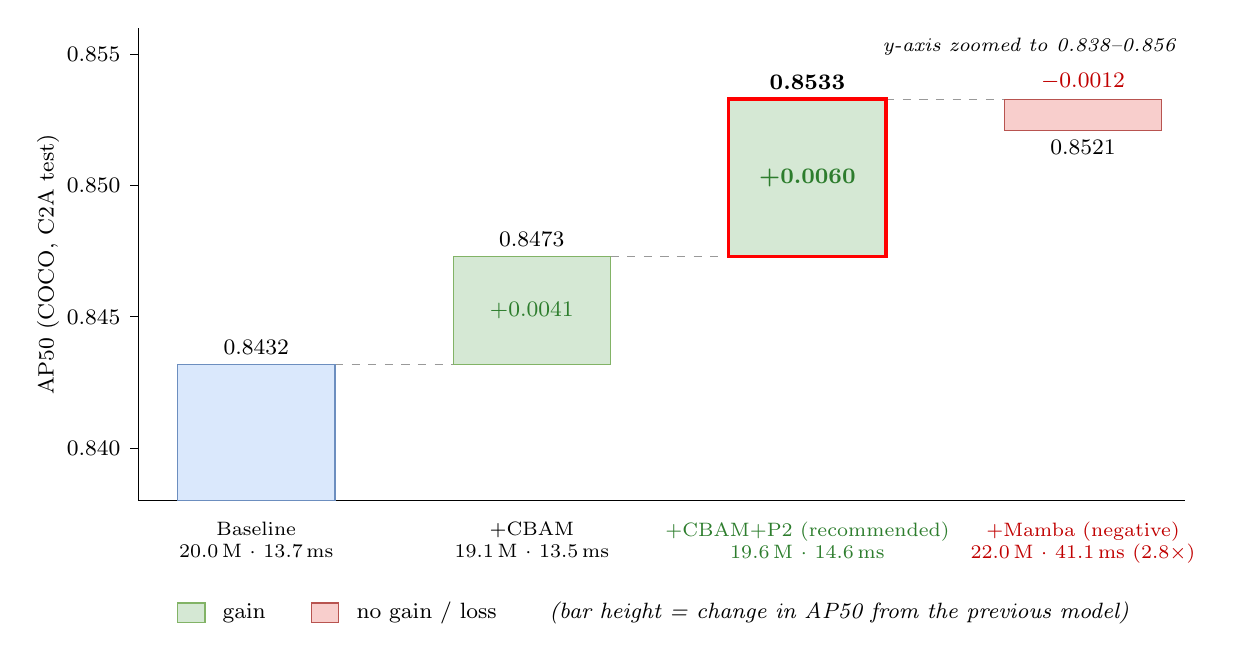
\begin{tikzpicture}[font=\footnotesize]
  % ---- axes ----
  \draw[black] (1.0,0) -- (1.0,6.0);
  \draw[black] (1.0,0) -- (14.3,0);
  \foreach \y/\lab in {0.6667/0.840, 2.3333/0.845, 4.0/0.850, 5.6667/0.855}{%
    \draw[black] (0.9,\y) -- (1.0,\y);
    \node[left] at (0.9,\y) {\lab};
  }
  \node[rotate=90,anchor=south] at (0.12,3.0) {AP50 (COCO, C2A test)};
  \node[anchor=north east,font=\itshape\scriptsize] at (14.3,6.0) {y-axis zoomed to 0.838--0.856};

  % ---- dashed step connectors ----
  \draw[wfGrey,dashed] (3.5,1.7333) -- (5.0,1.7333);
  \draw[wfGrey,dashed] (7.0,3.1)    -- (8.5,3.1);
  \draw[wfGrey,dashed] (10.5,5.1)   -- (12.0,5.1);

  % ---- bars ----
  \filldraw[fill=wfBaseFill,draw=wfBaseStroke]                     (1.5,0)      rectangle (3.5,1.7333);
  \filldraw[fill=wfGainFill,draw=wfGainStroke]                     (5.0,1.7333) rectangle (7.0,3.1);
  \filldraw[fill=wfGainFill,draw=wfRedEdge,line width=1.2pt]       (8.5,3.1)    rectangle (10.5,5.1);
  \filldraw[fill=wfMambaFill,draw=wfMambaStroke]                   (12.0,4.7)   rectangle (14.0,5.1);

  % ---- resulting AP50 above/below each bar ----
  \node[above] at (2.5,1.7333) {0.8432};
  \node[above] at (6.0,3.1)    {0.8473};
  \node[above,font=\footnotesize\bfseries] at (9.5,5.1) {0.8533};
  \node[below] at (13.0,4.7)   {0.8521};

  % ---- per-step delta ----
  \node[text=wfGreenText]                       at (6.0,2.4167) {+0.0041};
  \node[text=wfGreenText,font=\footnotesize\bfseries] at (9.5,4.1) {+0.0060};
  \node[above,text=wfRedText]                   at (13.0,5.1)   {$-0.0012$};

  % ---- x-axis labels: model, params, latency ----
  \node[below,align=center,font=\scriptsize] at (2.5,-0.15)
        {Baseline\\20.0\,M $\cdot$ 13.7\,ms};
  \node[below,align=center,font=\scriptsize] at (6.0,-0.15)
        {+CBAM\\19.1\,M $\cdot$ 13.5\,ms};
  \node[below,align=center,font=\scriptsize,text=wfGreenText] at (9.5,-0.15)
        {+CBAM+P2 (recommended)\\19.6\,M $\cdot$ 14.6\,ms};
  \node[below,align=center,font=\scriptsize,text=wfRedText] at (13.0,-0.15)
        {+Mamba (negative)\\22.0\,M $\cdot$ 41.1\,ms (2.8$\times$)};

  % ---- legend ----
  \filldraw[fill=wfGainFill,draw=wfGainStroke]  (1.5,-1.55) rectangle (1.85,-1.30);
  \node[anchor=west] at (1.95,-1.425) {gain};
  \filldraw[fill=wfMambaFill,draw=wfMambaStroke] (3.2,-1.55) rectangle (3.55,-1.30);
  \node[anchor=west] at (3.65,-1.425) {no gain / loss};
  \node[anchor=west,font=\footnotesize\itshape] at (6.1,-1.425) {(bar height = change in AP50 from the previous model)};
\end{tikzpicture}

%  y = (AP50 - 0.838) * 333.333 cm  (axis zoomed to 0.838-0.856)
% ============================================================================
\definecolor{wfBaseFill}{HTML}{DAE8FC}
\definecolor{wfBaseStroke}{HTML}{6C8EBF}
\definecolor{wfGainFill}{HTML}{D5E8D4}
\definecolor{wfGainStroke}{HTML}{82B366}
\definecolor{wfRedEdge}{HTML}{FF0000}
\definecolor{wfMambaFill}{HTML}{F8CECC}
\definecolor{wfMambaStroke}{HTML}{B85450}
\definecolor{wfGreenText}{HTML}{2D7D2D}
\definecolor{wfRedText}{HTML}{C00000}
\definecolor{wfGrey}{HTML}{999999}
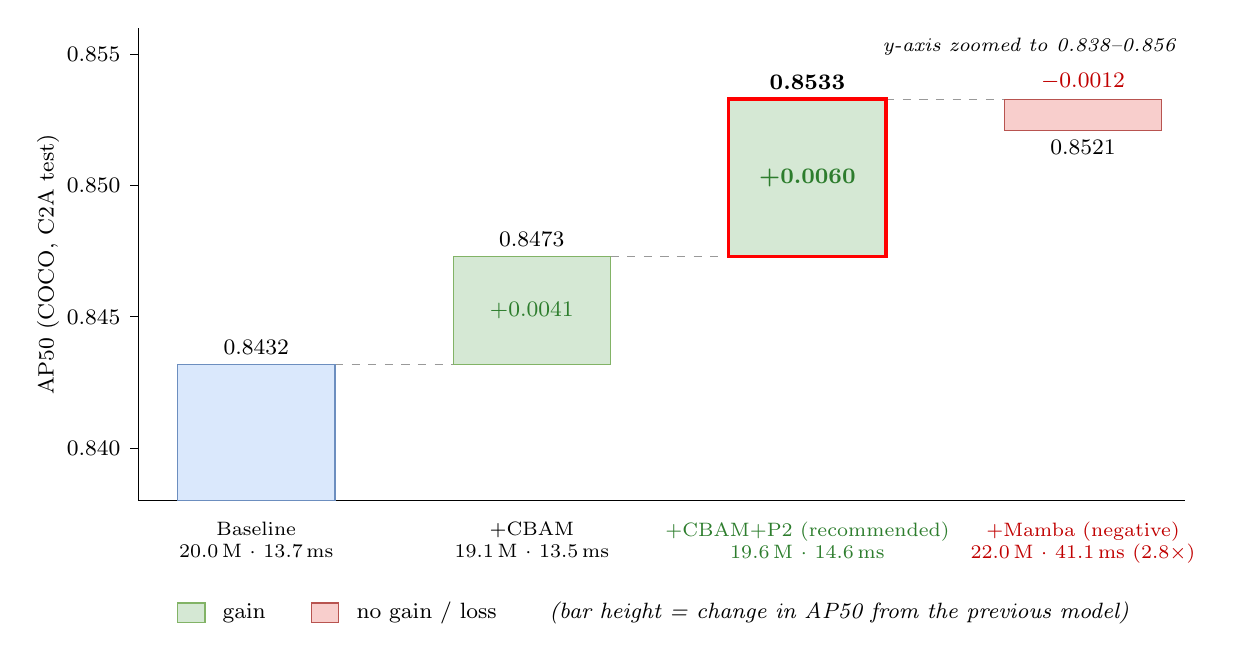
\begin{tikzpicture}[font=\footnotesize]
  % ---- axes ----
  \draw[black] (1.0,0) -- (1.0,6.0);
  \draw[black] (1.0,0) -- (14.3,0);
  \foreach \y/\lab in {0.6667/0.840, 2.3333/0.845, 4.0/0.850, 5.6667/0.855}{%
    \draw[black] (0.9,\y) -- (1.0,\y);
    \node[left] at (0.9,\y) {\lab};
  }
  \node[rotate=90,anchor=south] at (0.12,3.0) {AP50 (COCO, C2A test)};
  \node[anchor=north east,font=\itshape\scriptsize] at (14.3,6.0) {y-axis zoomed to 0.838--0.856};

  % ---- dashed step connectors ----
  \draw[wfGrey,dashed] (3.5,1.7333) -- (5.0,1.7333);
  \draw[wfGrey,dashed] (7.0,3.1)    -- (8.5,3.1);
  \draw[wfGrey,dashed] (10.5,5.1)   -- (12.0,5.1);

  % ---- bars ----
  \filldraw[fill=wfBaseFill,draw=wfBaseStroke]                     (1.5,0)      rectangle (3.5,1.7333);
  \filldraw[fill=wfGainFill,draw=wfGainStroke]                     (5.0,1.7333) rectangle (7.0,3.1);
  \filldraw[fill=wfGainFill,draw=wfRedEdge,line width=1.2pt]       (8.5,3.1)    rectangle (10.5,5.1);
  \filldraw[fill=wfMambaFill,draw=wfMambaStroke]                   (12.0,4.7)   rectangle (14.0,5.1);

  % ---- resulting AP50 above/below each bar ----
  \node[above] at (2.5,1.7333) {0.8432};
  \node[above] at (6.0,3.1)    {0.8473};
  \node[above,font=\footnotesize\bfseries] at (9.5,5.1) {0.8533};
  \node[below] at (13.0,4.7)   {0.8521};

  % ---- per-step delta ----
  \node[text=wfGreenText]                       at (6.0,2.4167) {+0.0041};
  \node[text=wfGreenText,font=\footnotesize\bfseries] at (9.5,4.1) {+0.0060};
  \node[above,text=wfRedText]                   at (13.0,5.1)   {$-0.0012$};

  % ---- x-axis labels: model, params, latency ----
  \node[below,align=center,font=\scriptsize] at (2.5,-0.15)
        {Baseline\\20.0\,M $\cdot$ 13.7\,ms};
  \node[below,align=center,font=\scriptsize] at (6.0,-0.15)
        {+CBAM\\19.1\,M $\cdot$ 13.5\,ms};
  \node[below,align=center,font=\scriptsize,text=wfGreenText] at (9.5,-0.15)
        {+CBAM+P2 (recommended)\\19.6\,M $\cdot$ 14.6\,ms};
  \node[below,align=center,font=\scriptsize,text=wfRedText] at (13.0,-0.15)
        {+Mamba (negative)\\22.0\,M $\cdot$ 41.1\,ms (2.8$\times$)};

  % ---- legend ----
  \filldraw[fill=wfGainFill,draw=wfGainStroke]  (1.5,-1.55) rectangle (1.85,-1.30);
  \node[anchor=west] at (1.95,-1.425) {gain};
  \filldraw[fill=wfMambaFill,draw=wfMambaStroke] (3.2,-1.55) rectangle (3.55,-1.30);
  \node[anchor=west] at (3.65,-1.425) {no gain / loss};
  \node[anchor=west,font=\footnotesize\itshape] at (6.1,-1.425) {(bar height = change in AP50 from the previous model)};
\end{tikzpicture}

  \caption{Contribution of each component to $\mathrm{AP}_{50}$ on the C2A test set
  (additive ablation; the $y$-axis is zoomed to $0.838$--$0.856$). Each bar is the
  change from the previous model; parameters and end-to-end latency are listed
  beneath each configuration.}
  \label{fig:waterfall}
\end{figure}

The per-size recall in Table~\ref{tab:persize} explains the aggregate flatness. The
P2 head raises very-tiny ($<8$~px) recall from $0.743$ to $0.757$ ($+1.5$~points),
the band that matters most for spotting distant victims, but it slightly lowers
recall in the tiny, small, and medium bands. The medium band drops most in relative
terms, but it contains only 317 of the roughly 72{,}500 test instances, so its
contribution to the aggregate is small and its estimate is noisy. The net effect is
a model that is better at the smallest targets and roughly even elsewhere, which is
the intended trade for this application. The state-space neck tracks CBAM~+~P2
almost exactly here, confirming it adds nothing in the size regime it was meant to
help.

\begin{table}[tbp]
  \centering
  \caption{Per-size recall on the C2A test set, by target pixel area. Ground-truth
  counts per band are shown; the medium band is small (317 instances) and its
  recall estimate is correspondingly noisy.}
  \label{tab:persize}
  \begin{tabular}{@{}l r r r r@{}}
    \toprule
    Model & very-tiny & tiny & small & medium \\
    & ($<8$px) & ($8$--$16$) & ($16$--$32$) & ($32$--$96$) \\
    GT instances & 25{,}072 & 20{,}520 & 26{,}614 & 317 \\
    \midrule
    YOLO11m baseline    & 0.743 & 0.869 & 0.894 & 0.909 \\
    + CBAM              & 0.746 & 0.873 & 0.895 & 0.912 \\
    + CBAM + P2         & \textbf{0.757} & 0.865 & 0.886 & 0.808 \\
    + Mamba + CBAM + P2 & \textbf{0.757} & 0.870 & 0.887 & 0.811 \\
    \bottomrule
  \end{tabular}
\end{table}

Figure~\ref{fig:curves} shows the precision--recall and $F_1$--confidence curves for
the recommended CBAM~+~P2 model, and Figure~\ref{fig:calib} its reliability
diagram; the expected calibration error is $0.021$, so the confidence scores are
close to their empirical accuracy. The per-epoch training curves are in
Figure~\ref{fig:training}.

\begin{figure}[tbp]
  \centering
  \begin{minipage}{0.49\linewidth}\centering
    \figorplaceholder{figures/cbam_p2_pr_curve.png}{6.0cm}
  \end{minipage}\hfill
  \begin{minipage}{0.49\linewidth}\centering
    \figorplaceholder{figures/cbam_p2_f1_conf.png}{6.0cm}
  \end{minipage}
  \caption{Recommended CBAM~+~P2 model on the C2A test set: (a)~precision--recall
  curve and (b)~$F_1$ score against confidence threshold, from which the operating
  point is chosen.}
  \label{fig:curves}
\end{figure}

\begin{figure}[tbp]
  \centering
  \begin{minipage}{0.49\linewidth}\centering
    \figorplaceholder{figures/cbam_p2_calibration.png}{6.0cm}
  \end{minipage}\hfill
  \begin{minipage}{0.49\linewidth}\centering
    \figorplaceholder{figures/cbam_p2_confusion.png}{6.0cm}
  \end{minipage}
  \caption{CBAM~+~P2 model: (a)~reliability diagram (expected calibration error
  $0.021$) and (b)~confusion matrix on the C2A test set.}
  \label{fig:calib}
\end{figure}

\begin{figure}[tbp]
  \centering
  \figorplaceholder{figures/cbam_p2_training_panel.png}{7.5cm}
  \caption{Per-epoch training and validation dynamics for the CBAM~+~P2 model: box,
  classification, and distribution-focal losses together with precision, recall,
  and mAP over the course of training.}
  \label{fig:training}
\end{figure}

\subsection{Qualitative Results and Error Analysis}
The per-size results in Table~\ref{tab:persize} show where the recommended model
still fails, and inspection of the missed detections groups them into three
recurring types. The first is heavy occlusion, where a person is mostly hidden by
debris or water and only a small fragment stays visible. The second is the
extreme-scale case, where a target spans only a few pixels and carries too little
texture to separate it from the background. The third is crowding, where several
people stand close together and the detector merges them into one box. These types
match the numbers. The very-tiny band holds the largest share of the residual
error, while the medium band, which contains few instances and larger targets, is
almost saturated. The trade the model makes is therefore the intended one for this
task: it recovers more of the smallest targets, where a missed detection is a missed
person, at a small cost on the easier size bands. Figure~\ref{fig:detgrid} makes the
scale argument concrete on a real cluster: the stride-8 (P3) grid assigns several
neighbouring people to a single cell, whereas the stride-4 (P2) grid separates them.

\begin{figure}[tbp]
  \centering
  \begin{minipage}{0.46\linewidth}\centering
    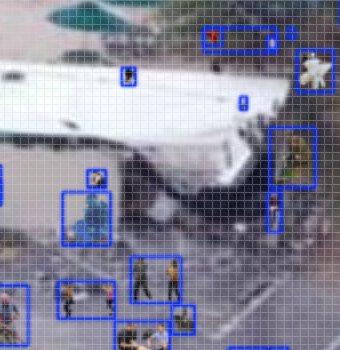
\includegraphics[width=\linewidth,height=5cm,keepaspectratio]{figures/detgrid_c2a_s8.png}\\[2pt]
    {\small (a) stride-8 (P3) grid}
  \end{minipage}\hfill
  \begin{minipage}{0.46\linewidth}\centering
    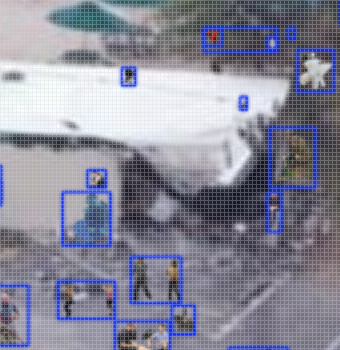
\includegraphics[width=\linewidth,height=5cm,keepaspectratio]{figures/detgrid_c2a_s4.png}\\[2pt]
    {\small (b) stride-4 (P2) grid}
  \end{minipage}
  \caption{Detection-cell granularity on a C2A cluster crop, with detected boxes
  overlaid: the stride-8 (P3) grid~(a) covers several neighbouring people per cell,
  whereas the stride-4 (P2) grid~(b) resolves them individually. This is the spatial
  reason the added P2 scale recovers more of the smallest targets.}
  \label{fig:detgrid}
\end{figure}

\subsection{Comparison with State-of-the-Art}
Table~\ref{tab:sota} places the recommended model against the published results of
Nihal et al.~\cite{nihal2024c2a} on the same C2A test split, none of which use
test-time slicing or augmentation. The CBAM~+~P2 model matches or exceeds every
convolutional and transformer baseline in that study except YOLOv9-e, and it does
so with about $19.6$~M parameters against YOLOv9-e's $57.3$~M, roughly a third of the
size. This compactness is the basis for the deployment discussion in
Section~\ref{sec:lightweight}.

\begin{table}[tbp]
  \centering
  \caption{Comparison with published detectors on the C2A test set. Baseline
  numbers are from Nihal et al.~\cite{nihal2024c2a}, which use standard training
  without slicing or test-time augmentation.}
  \label{tab:sota}
  \begin{tabular}{@{}l r r r@{}}
    \toprule
    Model & $\mathrm{AP}_{50}$ & AP & Params \\
    \midrule
    Faster R-CNN            & 0.634 & 0.366 & $\sim$41M \\
    RetinaNet               & 0.693 & 0.383 & $\sim$37M \\
    RTMDet                  & 0.708 & 0.442 & --- \\
    Cascade R-CNN           & 0.735 & 0.486 & $\sim$69M \\
    DINO                    & 0.789 & 0.471 & $\sim$47M \\
    YOLOv5                  & 0.808 & 0.492 & --- \\
    YOLOv9-e                & \textbf{0.893} & \textbf{0.688} & 57.3M \\
    \midrule
    YOLO11m baseline (ours) & 0.843 & 0.615 & 20.1M \\
    CBAM + P2 (ours)        & 0.853 & 0.615 & \textbf{19.6M} \\
    \bottomrule
  \end{tabular}
\end{table}

\subsection{Inference-Time Enhancement: SAHI and TTA}
Slicing-aided hyper inference (SAHI)~\cite{akyon2022sahi} runs the trained detector
over overlapping crops so that very small targets occupy a larger fraction of each
input tile; test-time augmentation (TTA) instead runs the detector at several
resolutions and merges the results. Both are applied to the recommended CBAM~+~P2
model as separate, clearly-labelled inference-time settings, not folded into the
primary table, because the sliced protocol uses per-image box matching for which the
standard mAP is not directly comparable. Table~\ref{tab:sahi} reports the sweep and
Figure~\ref{fig:sahibars} the resulting per-size recall. Among the SAHI settings, a
$256$-px slice gives the highest very-tiny recall, $0.788$ (up from $0.758$,
$+3.0$~points), but at $162$~ms per image; larger slices run faster
($54$--$113$~ms) and recover slightly less. Test-time augmentation at $1280$~px is
the most effective single setting: it raises very-tiny recall to $0.850$
($+9.2$~points) and the operational $F_2$ to $0.854$, and lifts mAP50 from $0.868$
to $0.878$ and mAP50-95 from $0.632$ to $0.677$, all at $60$~ms, cheaper than any
SAHI configuration. Beyond $1280$~px it degrades, as a model trained at $640$~px
cannot extrapolate to several times the resolution. Both remain optional
inference-time settings that trade latency for recall on the smallest targets;
neither is part of the primary model.

\begin{table}[tbp]
  \centering
  \caption{SAHI slice-size sweep and TTA on the C2A test set for the recommended
  CBAM~+~P2 model, reported as separate inference-time settings (per-image box
  matching at IoU~0.5; latency is the mean per-image time on the 4070 Ti SUPER). The
  baseline row is the same model at $640$~px without slicing or augmentation.}
  \label{tab:sahi}
  \setlength{\tabcolsep}{4pt}
  \begin{tabular}{@{}l r r r r r r r@{}}
    \toprule
    Setting & Size & $P$ & $R$ & $F_1$ & $F_2$ & very-tiny R & Lat.\ (ms) \\
    \midrule
    no SAHI (baseline) & 640  & 0.857 & 0.835 & 0.845 & 0.839 & 0.758 & 15 \\
    + SAHI             & 256  & 0.853 & 0.846 & 0.850 & 0.848 & 0.788 & 162 \\
    + SAHI             & 320  & 0.861 & 0.844 & \textbf{0.852} & 0.847 & 0.782 & 113 \\
    + SAHI             & 512  & 0.864 & 0.837 & 0.850 & 0.842 & 0.763 & 66 \\
    + SAHI             & 640  & 0.864 & 0.833 & 0.848 & 0.839 & 0.756 & 54 \\
    + TTA              & 1280 & 0.774 & 0.877 & 0.822 & \textbf{0.854} & \textbf{0.850} & 60 \\
    \bottomrule
  \end{tabular}
\end{table}

\begin{figure}[tbp]
  \centering
  \figorplaceholder{figures/per_size_recall_all_configs.png}{7cm}
  \caption{Per-size recall of the CBAM~+~P2 model under each inference-time setting
  (baseline, the SAHI slice sweep, and TTA at $1280$~px) on the C2A test set. The
  gains concentrate in the very-tiny and tiny bands, and TTA gives the largest
  very-tiny improvement.}
  \label{fig:sahibars}
\end{figure}

\subsection{Lightweight Variant}
\label{sec:lightweight}
The recommended CBAM~+~P2 model is already compact. At $19.6$~M parameters it is
smaller than the plain YOLO11m baseline and about a third the size of the largest
published detector on C2A, and it runs at $14.6$~ms per image on a single consumer
GPU, which is real-time for drone review at typical frame rates. For on-board use on
constrained hardware, the same recipe, meaning the CBAM substitution and the added
P2 scale, transfers directly to a smaller YOLO11 backbone such as YOLO11s, which
trades a little accuracy for a further cut in parameters and latency. Building that
variant and measuring it on an embedded device is set out as future work in
Chapter~VII; the design presented here is already small enough to deploy without it.

\section{Objective Achieved}
The objectives set in Chapter~I are met as follows. The additive ablation isolates
the contribution of each component and identifies CBAM~+~P2 as the configuration
that best serves the task, since it gives the best very-tiny recall and operational
$F_2$ at a parameter count below the baseline with P2 alone. The comparison in
Table~\ref{tab:sota} shows the model is competitive with published detectors on C2A
at a fraction of their size, which meets the objective of a compact,
deployment-ready detector. The state-space neck was evaluated honestly and shown not
to help, which answers the design question it was introduced to test.

\section{Financial Analyses and Budget}
The work used hardware already available and open-source software, so the direct
monetary cost is limited to electricity. Training the four configurations took
about 7--30 hours each on the 4070 Ti SUPER (the state-space model being the
longest at $29.5$~h), at an average board power of roughly $180$~W. The full set of
training runs therefore consumed on the order of $10$--$15$~kWh. No paid datasets,
cloud compute, or licences were required.

\section{Conclusion}
The additive ablation shows that the gain on C2A comes almost entirely from the P2
detection scale, which lifts very-tiny recall and $\mathrm{AP}_{50}$ at a small
cost, while CBAM contributes efficiency and the state-space neck contributes
nothing at a large latency cost. The recommended CBAM~+~P2 model is competitive with
much larger published detectors on the same data. The next chapters consider the
wider engineering context of the work and its conclusions.
